%%%%%%%%%%%%%%%%%%%%%%%%%%%%%%%%%%%%%%%%%%%%%%%%%%%%%%%%%%%%%%%%%%%%%%%%%%%%%%%%
%2345678901234567890123456789012345678901234567890123456789012345678901234567890
%        1         2         3         4         5         6         7         8


\documentclass[letterpaper, 10 pt, conference]{ieeeconf}  % Comment this line out
                                                          % if you need a4paper
%\documentclass[a4paper, 10pt, conference]{ieeeconf}      % Use this line for a4
                                                          % paper

\IEEEoverridecommandlockouts                              % This command is only
                                                          % needed if you want to
                                                          % use theplp \thanks command
\overrideIEEEmargins
% See the \addtolength command later in the file to balance the column lengths
% on the last page of the document



% The following packages can be found on http:\\www.ctan.org
\usepackage{graphics} % for pdf, bitmapped graphics files
\usepackage{epsfig} % for postscript graphics files
\usepackage{mathptmx} % assumes new font selection scheme installed
\usepackage{times} % assumes new font selection scheme installed
\usepackage{amsmath} % assumes amsmath package installed
\usepackage{amssymb}  % assumes amsmath package installed
\usepackage{mathtools}
\usepackage[noadjust]{cite}
\usepackage{dblfloatfix}
\usepackage{color}
\renewcommand{\thefigure}{\arabic{figure}}

\title{\LARGE \bf
A Novel Soft Elbow Exosuit to Supplement Bicep Lifting Capacity  
}

%\author{ \parbox{3 in}{\centering Huibert Kwakernaak*
%         \thanks{*Use the $\backslash$thanks command to put information here}\\
%         Faculty of Electrical Engineering, Mathematics and Computer Science\\
%         University of Twente\\
%         7500 AE Enschede, The Netherlands\\
%         {\tt\small h.kwakernaak@autsubmit.com}}
%         \hspace*{ 0.5 in}
%         \parbox{3 in}{ \centering Pradeep Misra**
%         \thanks{**The footnote marks may be inserted manually}\\
%        Department of Electrical Engineering \\
%         Wright State University\\
%         Dayton, OH 45435, USA\\
%         {\tt\small pmisra@cs.wright.edu}}
%}

\author{Carly M. Thalman, \textit{Student Member, IEEE}, Quoc P. Lam, Pham H. Nguyen, \textit{Student Member, IEEE}, 
\\Saivimal Sridar, \textit{Student Member, IEEE}, and Panagiotis Polygerinos$^{*}$, \textit{Member, IEEE}% <-this % stops a space
%\thanks{*Equally Contributing 1st Authors}% <-this % stops a space
\thanks{$*$ Corresponding Author}% <-this % stops a space
\thanks{Carly M. Thalman, Quoc P. Lam, Pham H. Nguyen, Saivimal Sridar, and Panagiotis Polygerinos are with the Polytechnic School, Ira A. Fulton Schools of Engineering, Arizona State University, Mesa, AZ 85212, USA.
        {\tt\small cmthalma@asu.edu, qlam1@asu.edu, nhpham2@asu.edu, ssridar@asu.edu, polygerinos@asu.edu}}%
}



\begin{document}



\maketitle
\thispagestyle{empty}
\pagestyle{empty}


%%%%%%%%%%%%%%%%%%%%%%%%%%%%%%%%%%%%%%%%%%%%%%%%%%%%%%%%%%%%%%%%%%%%%%%%%%%%%%%%
\begin{abstract}

This paper investigates the design of a soft elbow exosuit capable of providing supplemental lifting assistance by reducing muscle activity of the bicep muscle.  The aim is to improve the efficiency and endurance of workers who are tasked with repetitive lifting. The design consists of an array of pneumatically pressurized soft actuators, which are encased in nylon fabric that allows for a high force-to-weight ratio of 211.5${N}/{g}$. An analytical model governing the bending behavior of two consecutive actuators and torque generated by the exosuit is developed, with test results showing less than 10\% error from the theoretical model.  An elbow joint torque value of 27.6$N{\cdot}m$ is achieved at 300$kPa$, which is comparable to the 30$N{\cdot}m$ maximum set by OSHA requirements in the USA. Further testing with a healthy participant is performed using surface electromyography (sEMG) sensors and a motion capture system to assess the capabilities of the exosuit to provide active assistance to the bicep during isometric and concentric contractions. Measurable assistance to lifting is observed with minimal obstruction to the user's range of motion for all experiments. 

\end{abstract}

%%%%%%%%%%%%%%%%%%%%%%%%%%%%%%%%%%%%%%%%%%%%%%%%%%%%%%%%%%%%%%%%%%%%%%%%%%%%%%%%
\section{INTRODUCTION}

Freight, stock, and warehouse workers are required to perform strenuous and repetitive tasks such as packing, shelving, loading, and unloading goods on a daily basis. These repetitive motions can lead to muscle fatigue, as well as lower-back and upper-limb injuries that reduce productivity. Injuries in this line of work can cause musculoskeletal disorders (MSDs) as a result of improper lifting postures, repetitive high strain activities, and age-related factors \cite{BLS2017}.

According to the US Department of Labor in 2015, there were 376,190 cases (33\% of all injury cases) of MSDs caused by overexertion in lifting \cite{BLS2016}. Of all the occupations, laborers and freight, stock, and material movers were part of the highest number of injury cases \cite{BLS2016}. The cost of workplace injury in the USA alone is amounted to approximately \$190 billion and has resulted in over 1.1 million lost days of work \cite{Leigh2011}. There has also been a consistent increase in the age of the labor force since the beginning of the century and the category of workers 45 years old and over has grown from 34\% to 44\% of the total labor force \cite{Mislinski2017}. 

\begin{figure}[t!]
\centering
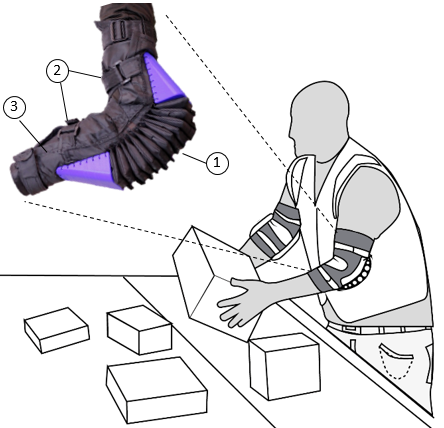
\includegraphics[width=0.45\textwidth]{Concept.PNG}
\caption{Illustrated concept of the soft robotic elbow exosuit in a warehouse environment. The physical prototype of the soft elbow exosuit is depicted in the expanded view.  Key design elements include: (1) Actuator array for flexion motion of elbow (2) Straps to tighten and loosen the elbow exosuit, (3) Elastic elbow sleeve to attach elbow exosuit to user’s arm. }
\label{fig:concept}
\vspace{-1.5em}
\end{figure}

Potential solutions for approaching this problem have been seen in the field of wearable robotics. These robotic devices are designed to help augment load carriage capacity and normal muscle function in healthy individuals while reducing the amount of physical exertion the user is required to sustain. Examples of human augmentation via exoskeletons have been seen for multi-purpose use in healthcare, rehabilitation, and industrial settings \cite{Kazerooni2008}. There have been a variety of lower-limb exoskeletons \cite{Viteckova2013} and upper-limb devices \cite{Gopura2016a}. These devices seek to increase the load bearing capability of the user. However, some of the primary concerns of using exoskeletons is:  rigidity, high development cost, portability, alignment complications with the biological joint they are trying to assist, and comfort over long periods of use.

The recent introduction and advancement of soft robotics has led to promising designs of wearable devices that are compliant, safe for human-robot interaction, lightweight, low-cost to fabricate, allow even distribution of force on the user's joints, and are less affected by alignment issues \cite{ADEM:ADEM201700016}. These intrinsically soft wearable devices have been categorized based on their novel form of actuation, including cable-driven actuators \cite{Gopura2016a,Dinh2017,Xiloyannis2017,Ding2016}, pneumatic artificial muscles \cite{Park2014cd,CALDWELL2007a,Al-fahaam2017}, fluidic elastomeric actuators\cite{Polygerinos,Koh2017,Chen2017h}, and pneumatically inflatable bladder-based actuators \cite{Kim2017,Sridar2017,Simpson2017,Koh2017}.
 
 In this paper the design and validation of a soft elbow exosuit utilizing a novel actuator array for bicep assistance during lifting is presented. \textcolor{black}{Figure \ref{fig:concept} illustrates the context in which the exosuit  is intended to be utilized.} Section II introduces the novel design of an inflatable actuator array as well its fabrication process.  An analytical model detailing the bending angle and torque generation of the exosuit is introduced in Section III.   Benchmarking and validation of the analytical models are presented in Section IV, while Section V evaluates the efficacy of the exosuit in participant testing.  

\section{DESIGN OF THE SOFT ELBOW EXOSUIT}

% Need to talk about ALL the individual parts of the exosuit, so that we can easily (and safely [Panos]) refer to them later in the text.
% actuator array, actuator (singular), sleeve, retainer/endcap, 

%A network of small cylindrical actuators (Fig. \ref{fig:array} (a) and (b)) are arranged in an array and when inflated,  interaction of the expanding actuators produces a bending motion.  The rotation is a result of the array being constrained along the base with an inextensible fabric (Fig. \ref{fig:array} (c) and (d)).
\begin{figure}[t]
\centering
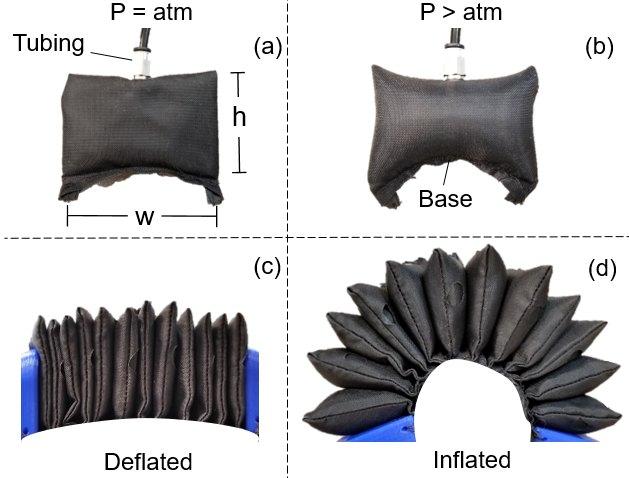
\includegraphics[width=0.4\textwidth]{V1_device.PNG}
\caption{(a) Deflated soft actuator with labeled dimensions for width, $w$ and height, $h$. (b) Inflated soft actuator. (c) Deflated soft actuator array. (d) Inflated soft actuator array.
}

\label{fig:array}
\end{figure}

The design of the soft elbow exosuit is based on a network of small, soft cylindrical actuators (Fig. \ref{fig:array}(a) and (b)) arranged in an array and constrained along the base with an inextensible fabric. When inflated, the individual actuators interact with one another other, to produce a bending motion as depicted in Fig. \ref{fig:array}(c) and (d).  

This methodology has been successfully proven to achieve predictable bending patterns using  individual actuators created by hermetically sealing the borders of two sheets of thermoplastic polyurethane (TPU) material \cite{ADEM:ADEM201700016,natividad2017h,Koh2017}. However, by encasing these actuators in an inextensible, weaved nylon material of the same net shape, the actuators can sustain higher pressures as they are no longer limited by the low tensile strength of the TPU during inflation.  This allows the soft actuators to obtain a higher force-to-weight ratio than previously possible. Previous work has implemented similar "bellow" actuator designs to assist human joints \cite{yamamoto2004stand}, however these solutions still rely on an entirely rigid frame.

%This allows for a novel approach to obtaining higher force-to-weight ratios from a single actuator than previously possible.



\begin{figure}
\centering
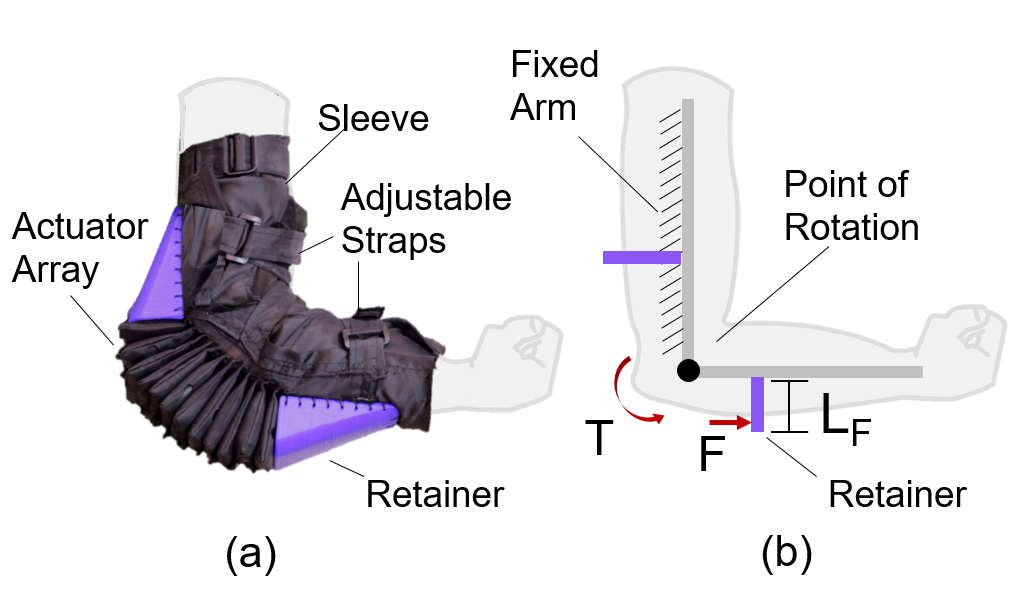
\includegraphics[width=0.45\textwidth]{arm.PNG}
\caption{Final Design of the soft robotic elbow sleeve (left) and the governing free body diagram (FBD) of the actuator array against the elbow (right)}
\label{fig:arm}
\vspace{-1.5em}
\end{figure}
 
 The bending of the soft actuator array is assumed to be constrained to the back of the elbow by a nylon fabric sleeve, which houses the components of the exosuit, as shown in Fig \ref{fig:arm}(a). The soft actuators at the end of the array are required to remain perpendicular to the arm in order to achieve the maximum torque output.  To achieve this, a triangular retainer is placed on either side of the array (Fig \ref{fig:arm}(a)). When pressurized, the actuators produces a bending moment given by:
\begin{equation}\label{torq}
	T = F{\cdot}L_F
    %T = \frac{P}{h{\cdot}w}L_F = 
\end{equation}


where, $T$ is the torque produced about the joint, $F$ is the generated force by pressurization of the soft actuator array and applied at a height of $L_F$ from the user's arm where the ends of the array contact the edge of the retainer as shown in Fig. \ref{fig:arm}(a) and (b).  The force $F$ is determined by the contact area between the soft actuator and retainer, $h{\cdot}w$ and the internal pressure.

%The average male, aged 24.4 $\pm$ 2.2 years, is capable of producing an average of 60 $N{\cdot}m$ of torque, at a 90$^o$ bend \cite{sardelli2011functional}. For the average female, this torque value is a maximum of 34 $N{\cdot}m$ a, or approximately half that of the average male \cite{laksanacharoen2003design}. Rather than design the exosuit to accommodate specific individuals, the exosuit is designed to assist for the safe maximum threshold set by OSHA requirements in the US, which is roughly $11kg$ per arm, or   $30 N\cdot{m}$, of torque \cite{waters1994applications} .%

  % include L_F as the moment arm in fig with the super buff arm. move the "retainer" (end-stop, can discuss the new name if you want)  outside the arm, it's inside rn. Need to add exosuit, and "sleeve" label, this is the first time it is introduced. We have just transitioned into calling it the exosuit! 
Keeping the safe maximum Occupational Safety and Health Administration (OSHA) requirements as noted in \cite{waters1994applications}, the exosuit is designed to provide 30$N{\cdot}m$ of torque about the elbow joint to assist the bicep. A lightweight, fabric-based design \cite{Sridar2017} is implemented through the use of compliant and soft materials. The base of each soft actuator is designed to fit the curvature of arm as shown in Fig \ref{fig:array}(b), which ensures the forces are applied over a distributed area. Adjustable hook and loop straps secure the fabric sleeve to the arm without covering the elbow crease. By adjusting the straps, the actuator array is secured against the curvature of the elbow joint so that it does not dislodge from the joint when inflated.

% The triangular retainers seen in Fig. \ref{fig:array}(a) serves to transmit the bending force generated by the actuator array over a larger contact area on the arm.

%\textcolor{red}{We should come back to organize this paragraph later. Content is there and just needs organization}

% Let's redo this section - what weight will begin to impact the user if they feel it?  For the grasper stuff I did way back it was about 300g I think before the user started to detect a difference. Maybe we can phase it that way.
%To keep the exosuit design lightweight, an upper limit of 2.3 kg is set - the average weight of the male forearm and hand combined \cite{clauser1969weight}. 

 \subsection{Fabrication}
The TPU  (DT-2001, American Polyfilm, Branford, CT) is sealed using a custom CNC router with a modified soldering iron tip set at $320^{\circ} C$ to trace and seal the complex contours of the soft actuators. A laser cutter (Glowforge Pro, Glowforge, Seattle, WA) is used to cut the outer nylon material pouches into the desired shape. It is then sewn into its final shape with the use of a sewing machine (SE-400 Brother, Bridgewater, NJ). The minimum distance between the soft actuators is limited to 5$mm$ due to manufacturing constraints of the sewing machine, which does not accurately enable a placement closer than this tolerance for the given configuration of the array. The height of each soft actuator is also restricted to a maximum of 50$mm$ in order to have a compact, low-profile exosuit.   
 
% Increase of variance in tolerances is a result of closely placed actuators, therefore a minimum distance of $5mm$ between actuators was set.  The height of  each actuator is constrained to a maximum of $50mm$, as any additional height is presumed to exceed a low-profile exosuit. The height of each actuator restricted to $50mm$ to 

\section{Theoretical Modeling}

\subsection{Modeling Free Space Bending Angle}

To model the bending curvature of the actuator array, the cross-section of two adjacent individual actuators is simplified to two dimensions as seen in Fig. \ref{fig:Model1}. When deflated, the actuators have no interaction with adjacent actuators in the array, as shown in Fig. \ref{fig:Model1}(a). The interaction between two actuators is modeled using the following assumptions:  $i)$ the individual actuators inflate to create a circular cross section, $ii)$ the deformation when fully pressurized is negligible, $iii)$ a point contact will form with adjacent actuators; and $iv)$ the actuators are fixed at a point to the inextensible layer (Fig. \ref{fig:Model1}(b)). The bending behavior of adjacent actuators is defined as: 
\begin{equation}\label{eq. sin}
	\theta_{actuator}=sin^{-1}(1-\frac{d}{2R}) 
\end{equation}

\begin{figure}[t!]
\centering
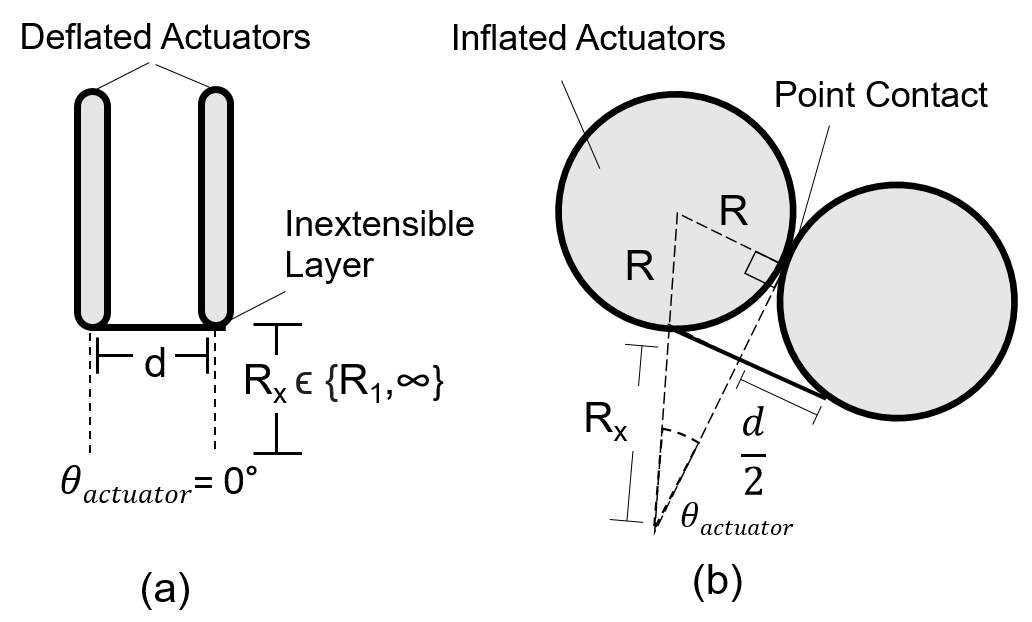
\includegraphics[width=0.4\textwidth]{ActuatorModel1.PNG}
\caption{(a) Model of two adjacent soft actuators in a deflated state, where no contact occurs.  (b) Two-dimensional geometric model of two adjacent soft actuators are fully pressurized.}
\label{fig:Model1}
\vspace{-1.5em}
\end{figure}

\begin{figure}[b!]
\centering
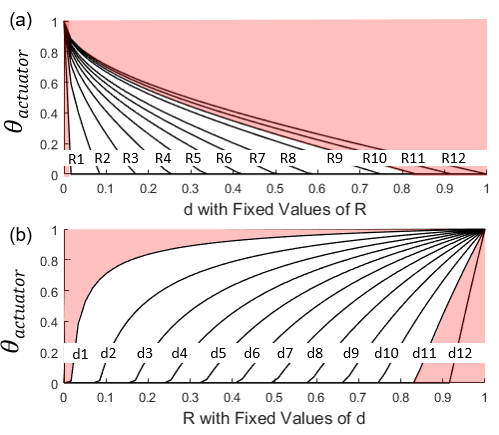
\includegraphics[width=0.45\textwidth]{graphs_model1.PNG}
\caption{All information presented in graphs has been normalized from $0^o$ to $90^o$, for $d$ and $R$.  (a) shows the relationship between $\theta_{actuator}$ and $d$ for incremental values of $R$.  (b) shows the relationship between $\theta_{actuator}$ and a varying $d$ given a fixed $R$. The shaded areas are unfeasible regions due to the previously mentioned manufacturing constraints of the sewing machine.}
\label{fig:Graphs1}

\end{figure}	
where,  $\theta_{actuator}$ is the bending caused by the interaction of adjacent soft actuators,  $d$ is the spacing between them, and $R$ is the radius of a single inflated actuator. A boundary condition of $ 2R > d$ is implemented to ensure that the interaction between two adjacent actuators causes bending for every considered value of  $\theta_{actuator}$.   

To determine the optimal parameters to achieve maximized bending angles, the $R$ and $d$ values are plotted separately by setting one of the parameters as a constant each time. Figure \ref{fig:Graphs1}(a) shows the variation in bending angles with constant $R$ values whereas Fig. \ref{fig:Graphs1}(b) shows the the same with constant values of $d$. It is observed that $\theta_{actuator}$ increases with both the decrease in $d$ and increase in $R$. Feasible regions for both $R$ and $d$ are identified by imposing the aforementioned manufacturing constraints depicted by the unshaded regions in Fig. \ref{fig:Graphs1}. Possible angles between two actuators have been limited to $90^{\circ}$ as the bending angle becomes asymptotic as $d$ becomes infinitely small. The angle $\theta_{actuator}$, represents the angle between the center of an actuator and its edge. It is equivalent to $\theta_{array}/2n$, where $\theta_{array}$ is the elbow angle and $n$, the number of soft actuators in the array. 

%PUT BACK LATER (???)  ranging from 12.5mm to 16mm based on the height of a flattened actuator to achieve height (40mm and the maximum height of 50mm respectively).  Based on these values, $d$ will be minimized \textcolor{red}{d has no dependency on R}.

\subsection{Modeling Torque Output}

%\begin{equation}\label{eq. X16}
%	F = PLw 
%\end{equation}

% need to talk about pressure force length and width in the design section. keep high high level, only enough for the reader to understand the thought process behind torque generation

\begin{figure}[t!]
\centering
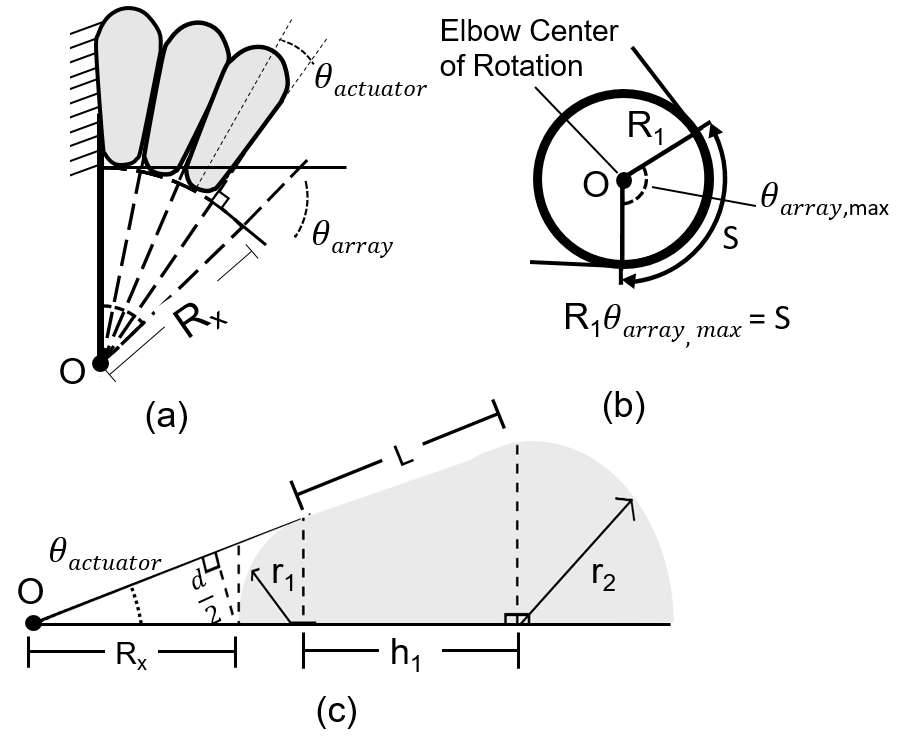
\includegraphics[width=0.45\textwidth]{model3.PNG}
\caption{(a) Simple bladder arrangement demonstrating interactions in the array.  (b) Spherical elbow joint representation of constant radius. $S$. The length of the actuator array is defined with this model. (c) Section view of an individual actuator depicting dimensions used in calculating the interacting area. }
\label{fig:hotness}
\end{figure}
%\textcolor{red}{S=R1theta0 and theta1 is centerline to interacting edge }

Modeling the torque output of the soft actuator array follows the same geometric principles outlined in Section IIIA. However, line contact across two actuators is replaced with the interacting area to account for shape deformation. Additionally, the array is no longer considered in free space bending, but constrained to the elbow joint. The resultant shape of the inflated soft actuators is shown in Fig \ref{fig:hotness}(a).  

The total length of the actuator array is represented by:
\begin{equation}\label{S}
	S = R_1\cdot\theta_{array,max}
\end{equation} 
where,  $S$ is the arc length, $R_1$ is the radius of the presumed spherical elbow joint, and  $\theta_{array,max}$ is the maximum bending angle of the elbow (Fig. \ref{fig:hotness}(b)). As torque is dependent on the moment arm $L_F$, as seen in (\ref{torq}), any additional length and/or number of actuators past the retainer has no effect on the torque output.

As a result of the actuator array bending with the elbow, $S$ bends as well with its radius of curvature defined as:

\begin{equation}\label{Rx2}
	R_x(\theta_{array}) = R_1\frac{\theta_{array,max}}{\theta_{array}}
\end{equation}
where $R_x$, is  the radius of curvature at the current angle, $\theta_{array}$.  Equation (\ref{Rx2}) demonstrates that $R_x$ can range from $R_1$ to ${\infty}$, which is portrayed in Fig. \ref{fig:Model1}(a).
% TMI - Figure \textcolor{red}{BOOM B} demonstrates that the range of $R_x$ must vary from ${\infty}$ to $R_{1}$ as the elbow bends from full extension through its full range of motion as it has an inverse dependence on $\theta_0$.   
% At $\theta_{max}$, $R_x$ is equal to $R_1$, therefore the same relationship is used to define the curvature radius  as bending angle varies through the elbow's flexion and extension. 


%Since the actuators are symmetrical about the radial centerline, the cross-section, shown in Fig. \ref{fig:hotness}(c), is used to extract remaining dimensions needed to calculate their reaction forces, i.e. $L$ and $w$.

%\textcolor{red}{replace L1 with h1 spanning the entire length of the actuator (at the bottom)}. That is not theta1 }

Upon closer inspection of the individual soft actuator, it can be observed that the shape resembles that of a right triangle with a quarter circle attached to the end (Fig. \ref{fig:hotness}(c)).  Using this shape as the foundation for the following torque model, we define the required dimensions needed to calculate the reaction force of the actuators of Eq. \ref{torq}. Using the tangent relationship, the  minor radius, $r_1$ is determined to be: 

\begin{equation}\label{r1}
	r_1(\theta_{actuator})  = \frac{d}{2cos(\theta_{actuator})}.
\end{equation}

While the major radius, $r_2$, also utilizes the tangent, the solution is expressed as
 \begin{equation}\label{r2}
	r_2(\theta_{actuator})  = -b + \sqrt{\frac{b^2-4ac}{2a}} ,
\end{equation}
where $a$, $b$, and $c$ are defined by

\begin{equation}\label{a}
	a = 1+\frac{1}{(\pi R+\sqrt{(R_x+r_1)^2+r_1^2})^2}+(\frac{\pi}{2})^2 ,
\end{equation}
\begin{equation}\label{a}
	b = \pi^2R+\pi\sqrt{(R_x+r_1)^2+r_1^2}-\frac{\pi^2r_1}{2} ,
\end{equation}
\begin{equation}\label{a}
\begin{aligned}
\begin{multlined}
	c = (\pi R+\sqrt{(R_x+r_1)^2+r_1^2})^2- (\pi R+\lambda)^2...\\\\
   +\pi^2Rr_1-(\frac{\pi R}{2})^2+\sqrt{(R_x+r_q)^2+r_1^2}\pi r_1 .
    \end{multlined}
    \end{aligned}
\end{equation}

To obtain the length of interaction, $L$, the perimeter length of a semi-circle is used to define the relationship between $L$ and the minor and major radius, $r_1$ and $r_2$, respectively, as shown: 
\begin{equation}\label{L}
	L(\theta_{actuator})  = \frac{\pi}{2}(r_1+r_2) -\pi R
\end{equation}

%Equations \textcolor{red}{BOOM} and \textcolor{red}{BOOM} is input into Eq. \textcolor{red}{BOOM BOOM} to find the $L$. 

assuming a constant width, $w$, as discussed in Section II. However, this does not provide a sufficient representation of the final inflated soft actuator. The actuators do not retain the same longitudinal cross-section dimensions when pressurized, witnessed in previous work and studies conducted on inflatable actuators \cite{natividad2017h}. Therefore, an adjusted effective width is required to better represent the behavior of the soft actuators:

\begin{equation}\label{w1}
	w_1(\theta_{actuator})  = w_0-2R(1-\frac{h_1(\theta_{actuator})-2R}{h-2R})
\end{equation}
where, $w_1$ represents the adjusted effective width of the actuator and $h_1$ represents the variable height. Utilizing (\ref{L}) and (\ref{w1}) to measure the effective area of interaction, a bending angle of 90$^{\circ}$ degrees is used as the variable input into the equation below to calculate the theoretical torque ($T$) generated by the exosuit:

\begin{equation}\label{torque}
	T(\theta_{actuator}) = PLL_Fw_1
\end{equation}

where, $P$ is the pressure input parameter and $L_F$ remains as defined in Eq. \ref{torq}. 


 %Therfore, an approximation is made on the effective width, $w_1$, in contact. It was assumed that reduction from initial width, $w_0$, is dependent on the ratio of the inflated actuator's height, $h_1$ to initial height, $h_0$ (eq. 8). 

%Once $\textit{L}$ was determined, the effective force was calculated, and therefore, the torque it would generate about the elbow joint. Since pressure, $\textit{P}$ is equal at every point within the inside of the actuator, force, $\textit{F}$ is also distributed evenly across the interacting area ($L\cdot w_{1}$) and is represented as a point load applied at $L_f$, the distance from the axis of rotation to the center of $L$.

%Various inputs, i.e. actuator heights, quantity of actuators and a 90 degree bending angle, were used to assess their resultant torque values (Fig. 8). The three main considerations for inputs were based on design constraints in which the remaining parameters are derived from them. Pressure input, $P$,  was set to a safe limit determined through preliminary testing of individual actuators, with reliable resistance to bursting up to 275kPa. Torque and pressure have linear dependencies as shown in Eq.  9 and 10, therefore only one set pressure was modeled for. 

The torque output of the actuator array is plotted against the number of individual actuators for fixed $h$ as shown in Fig \ref{fig:dif_R_n}. An increasing soft actuator radii, $R$ results in improved torque with diminishing returns from increasing the number of actuators, $n$. Using the set 30$N{\cdot}m$ as the minimum desired threshold and limiting the maximum pressure to 300$kPa$ for safety consideration. Fig. 7 suggests multiple design parameters that can be selected to generate a balance between manufacturability and ergonomics. As a result, we select a spacing,  $d$=8$mm$, number of actuators, $n$=12, and deflated actuator height, $h$=44$mm$. The width of the actuator is constrained to $w$=75$mm$ to fit the diameter of an average adult arm.


\begin{figure}[t!]
\centering
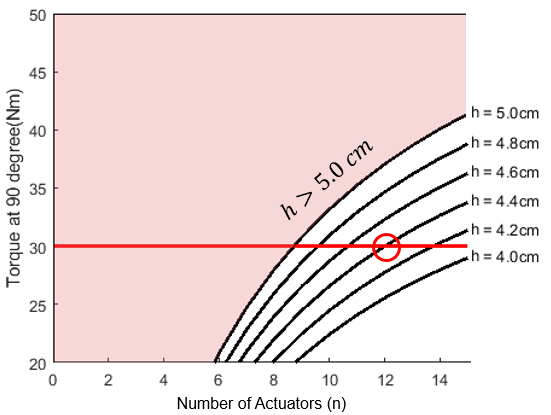
\includegraphics[width=0.4\textwidth]{dif_R_n.PNG}
\caption{Various actuator heights ($h$) and quantities ($n$) plotted to assess potential solutions to finding the optimum parameters that would yield 30$N{\cdot}m$ of torque.  The shaded regions indicated infeasible regions attributed to the aforementioned manufacturing constraints.}
\label{fig:dif_R_n}
\vspace{-1em}
\end{figure}



\section{EXPERIMENTAL METHODS AND RESULTS}

\subsection{Soft Actuator Stiffness}
\begin{figure}[t!]
\centering
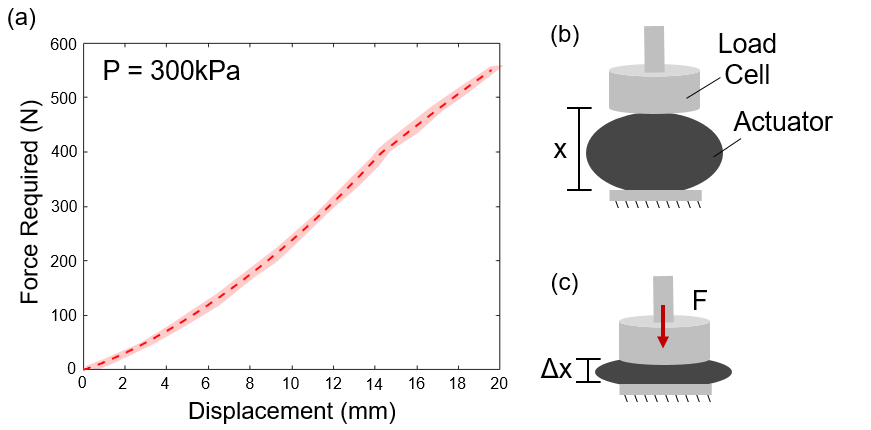
\includegraphics[width=0.48\textwidth]{stiiffnesstest.PNG}
\caption{Testing of an individual actuator to determine stiffness when fully pressurized (a) Displacement of the actuator and the corresponding force required to cause displacement.(b) Actuator in the UTM before compression, (c) and actuator in the UTM after compression}
\label{fig:stifftest}
\vspace{-1.5em}
\end{figure}

A single soft actuator is placed between compression platens of a universal tensile strength machine (UTM) (Instron 5944, Instron Corp., High Wycombe, United Kingdom) to determine its  stiffness.  The soft actuator is inflated up to a pressure of 300$kPa$ (as per the design parameters) and compressed to a total displacement of 19.5 $mm$, to the spacing between two adjacent actuators. The pressure is  held constant for the entirety of the test. A high force to weight ratio of 211.5${N}/{g}$ is obtained, given a single actuator weight of 2.6$g$ and a force output of 550$N$ for a single soft actuator (excluding tubing, connectors and power source).  A calculated stiffness of 28.2 $kN/m$ is found as a result of the maximum displacement and force obtained.

\subsection{Torque Verification}


\begin{figure} [t!]
\centering
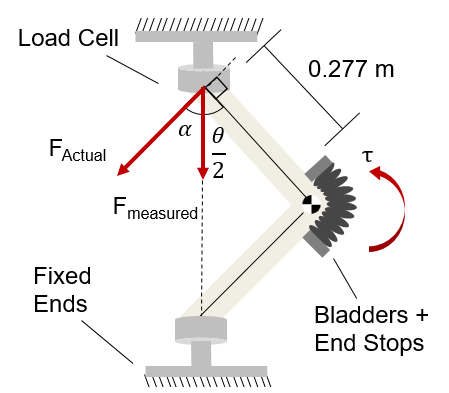
\includegraphics[width=0.3\textwidth]{torquetest.PNG}
\caption{Setup of torque test, showing the soft exosuit strapped to the analog joint while fixed in the UTM. }
\label{fig:t_test}
\end{figure}

\begin{figure}
\centering
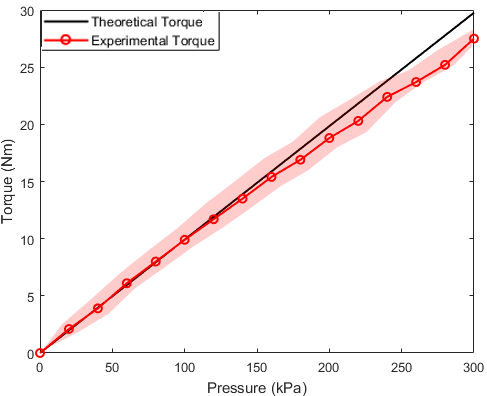
\includegraphics[width=0.4\textwidth]{Torque_stuff3.PNG}
\caption{Results of five trials for the torque test, displaying a linear relationship between the predicted torque values and the measured torque output of the exosuit.}
\label{fig:torques}
\vspace{-1em}
\end{figure}

To verify the torque output compared to the theoretical model shown in (\ref{torque}), the exosuit is secured to an analog elbow joint and placed in a UTM, with the joint angle fixed at $90^o$ (Fig. \ref{fig:t_test}). The actuator array is inflated in increments of 20$kPa$ up to a maximum of 300$kPa$ for five trials.  A linear trend is observed for the relationship between pressure and torque (r-squared of 0.99) as seen in Fig. \ref{fig:torques}. The linear regression model is compared to the theoretical model, and an average error of approximately 6.6\% is observed.  Overall, a maximum experimental torque of  27.1$\pm$0.67 $N\cdot m$ at a fixed  $90^{\circ}$ angle and 300$kPa$ is obtained in contrast to the estimated 30 $N{\cdot}m$, validating the accuracy of the model.

\section{PARTICIPANT TESTING}

In order to quantify the performance of the soft elbow exosuit, participant testing is performed with a healthy female participant (age: 23 years old, height: 1.67 m, weight: 52 kg, distance from elbow to center of palm: 0.32m). Surface electromyography measurement (sEMG) (Delsys® Trigno®, Delsys, Natick, MA) and motion capture (T40s, VICON Inc., Los Angeles, CA) are utilized for recording muscle activity of the bicep and bending angle of the elbow, respectively. Two experiments are performed with and without assistance from the exosuit. A total of three trials for each experiment are performed with two minute resting intervals between trials.

%\textcolor{red}{Each lift was timed for a total of two seconds lift, and two seconds release.} 

\begin{figure*}[t]
\centering
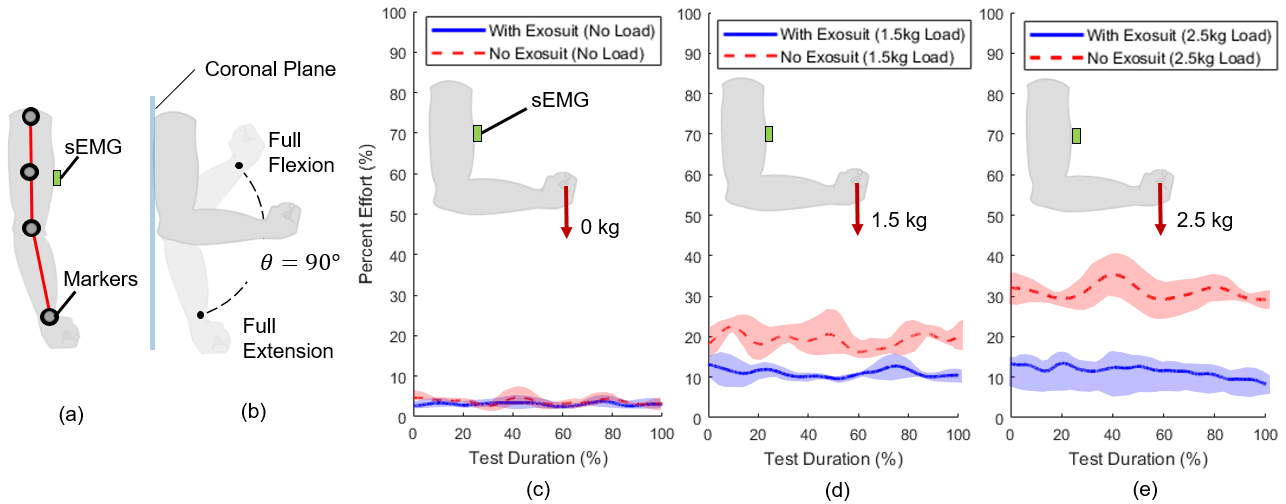
\includegraphics[width=0.95\textwidth]{EMG_Stuff2.PNG}
\caption{(a) Surface electromyography sensor and motion capture markers placement. (b) The measured positions of the arm for participant testing. (c) Baseline isometric muscle activity with no load. (d) Measured isometric muscle activity of bicep with a 1.5kg load (e) measured muscle activity of bicep with a 2.5kg load.}
\label{fig:EMG}
\vspace{-1em}
\end{figure*}

An sEMG sensor is placed at the bicep of the participant, shown in Fig. \ref{fig:EMG}(a), to measure muscle activity during the trials. The maximum voluntary contraction (MVC) and the muscle activity during relaxation is collected as per standard  International Society of Electrophysiology and Kinesiology (ISEK) protocols \cite{2018I}. The MVC limit is measured with the participant exerting maximum force against the load cell of the UTM with their elbow at a 90$^{\circ}$ bend, and their upper arm lying on the coronal plane (Fig. \ref{fig:EMG}(b)). Three individual tests are recorded, which result in an average maximum load of 73.6$\pm$9$N$ (7.5$\pm$0.9$kg$) of force exerted by the participant.  This value is considered the maximum load the participant can support at $90^o$. The current control method of exosuit actuation is built on a single-input-single-output (SISO) open loop system. Pressure is manually defined and monitored by an adjustable analog pneumatic regulator.

\subsection{Assisted Lift Test}
The lifting assistance provided by the exosuit is verified by repeating the procedure of flexing the arm from full extension to a fixed elbow joint angle position at 90$^o$ and holding the arm there for five seconds before relaxing back to full extension. The isometric contractions (i.e. muscle contractions while the arm does not move) of the bicep are monitored.  Initially, a baseline for the isometric contraction of the participant's bicep is established by recording the sEMG activity while performing the procedure without load, with and without assistance from the exosuit (Fig. \ref{fig:EMG}(c)). The same procedure is then repeated for varying load of 1.5$kg$ and 2.5$kg$, first without then with assistance as shown in Fig. \ref{fig:EMG}(d) and (e).  

The sEMG data is normalized with respect to the MVC and shows the unassisted isometric contractions for the 1.5kg load to be 19.2\% of the participant's MVC, and 31.2\% of the MVC for the 2.5kg load. It is observed that the averaged exosuit assistance provides 43\% and 63\% reduction in the activity of the bicep during the static test, as shown in Fig \ref{fig:EMG} (d) and (e). The sEMG data in Fig. \ref{fig:EMG} (d) and (e) indicate that there is residual muscle activity present even when assistance is provided by the exosuit possibly due to the effects of the participant straining to prevent unwanted wrist extension.

\subsection{Range of Motion (ROM) Study}

\begin{figure}[t!]
\centering
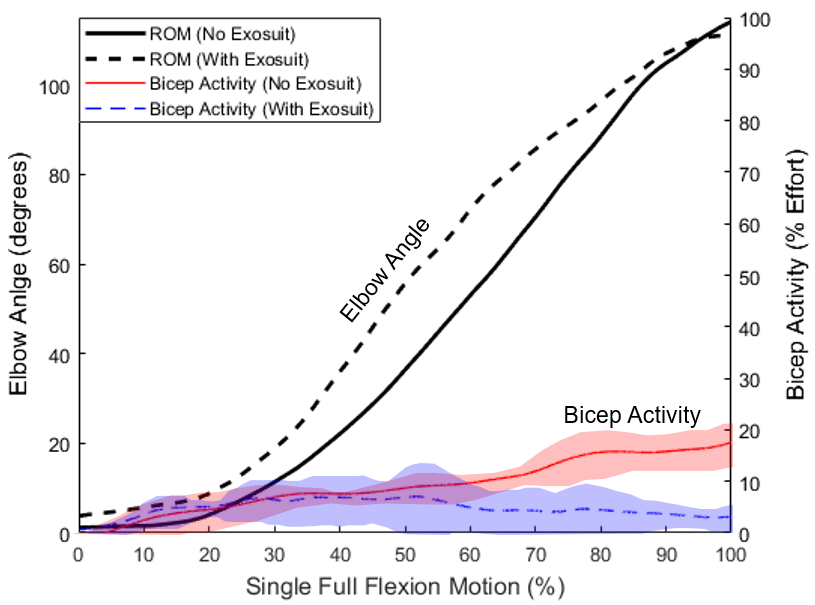
\includegraphics[width=0.45\textwidth]{ROM.PNG}
\caption{Range of Motion of the participant with and without wearing the device from  $0^o$  (full extension) to $115^o$(full flextion) is shown on the vertical axis on the left.  sEMG data during motion is shown on the right. 
}
\label{fig:ROM}
\vspace{-1.5em}
\end{figure}

A test is performed to quantify whether the participant's ROM may be affected by the exosuit. The sEMG sensor is used to monitor the concentric contractions (i.e. muscle contraction during arm motion) of the bicep from full extension to full flexion for signs of assistance through muscle activity reduction. Passive reflective markers are placed at the top of the shoulder (acromion), center of upper arm (humerus), elbow’s axis of rotation (medial epicondyle), and wrist (styloid process) (Fig. \ref{fig:EMG}(b)) to allow the motion capture system to track the motion during a single bicep curl. The participant  performs a single curl with no assistance from the exosuit, then repeats the motion relying on only the exosuit to achieve full flexion. Three trials are recorded with the upper arm remaining parallel to the coronal plane throughout the experiment. The observed angle at the elbow joint and corresponding bicep activity is shown in Fig. \ref{fig:ROM}.

The total elbow angle prior to wearing the exosuit spans $115^o \pm 4^o$ from full extension to full flexion. The range of motion while wearing the device is found to be $107^o \pm 8^o$. This verifies that the exosuit does not obstruct  $93\%$ of the the ROM.  Additionally, a reduction of 47\% in the muscle activity of the bicep is observed throughout the entire motion when the exouit is assisting.  This validates that the exosuit is capable of providing active assistance to the bicep through the entire motion.

\section{CONCLUSIONS}

In this paper, the design, characterization, and evaluation of a lightweight, soft elbow exosuit aimed to assist in elbow flexion of warehouse workers was presented. Such a design has the potential to be utilized by warehouse workers to reduce muscle strain and injuries. The exosuit is composed of an array of overlapping TPU based actuators enclosed in an inelastic fabric pouch in order to  withstand higher pressures, and therefore produced more force.  The individual actuators were designed with a curved base to match the curvature of the arm. 

The actuators were tested and characterized for stiffness, and the final actuator array was tested for torque generation at the elbow joint. It was observed that a single actuator can achieve high stiffness (28.2$kN/m$), with a force-to-weight ratio of 211.5$N/g$. The array of actuators was able to perform the primary task of providing 27.6$ N{\cdot}m$ of torque about about the elbow at $90^o$. Retainers were placed on either ends of the array to transmit forces to the body and to maintain the actuators perpendicular to the surface of the arm. It was observed that slight slippage of the straps at higher pressures had a tendency to cause loss in overall torque output.

A participant was recruited to assess the efficacy of the exosuit, with and without assistance while carrying different loads (1.5kg and 2.5kg). It was demonstrated that the exosuit was successful in providing assistance during isometric contractions of the bicep through the duration of a static test where the elbow was held at $90^o$. The results of the processed sEMG data showed a 43\% reduction in muscle activity for the 1.5kg weight and 63\% reduction for the 2.5kg weight when the device was active. The exosuit also demonstrated  the ability to maintain 93\% of the original ROM during full extension to flexion of the elbow.  It was also shown to provide assistance through the entire ROM with no load and an average of 47\% muscle activity reduction with the exosuit active. 

Future work will include incorporation of soft inflatable retainers on the ends of the array and improving the securing straps for increased comfort and better force distribution while preventing slippage against the skin.  Initial participant testing indicated that wider straps would help further increase the comfort of the device when used at higher pressures. Force and pressure control will be implemented for more precise actuation of the exosuit, as well as user intent detection for lifting objects.  The speed of actuation will be assessed in future work, as it is variable and dependent on the flow rate at the pressure source, as well as the size tubing used for the exosuit. An additional actuator will be incorporated to assist in the extension motion of the elbow and provide stiffness to support the joint during heavy lifting. Furthermore, investigation of the performance variations and design of the actuators through computational finite-element method (FEM) modeling will be explored to fully optimize each parameter for different orientation, as well as different material performance for the soft actuator array.  Finally, testing with a larger sample of participants for more comprehensive results will be performed.  


%%%%%%%%%%%%%%%%%%%%%%%%%%%%%%%%%%%%%%%%%%%%%%%%%%%%%%%%%%%%%%%%%%%%%%%%%%%%%%%%

\section*{ACKNOWLEDGMENTS}
C.M. Thalman is funded by the National Science Foundation Graduate Research Fellowships Program.  

%%%%%%%%%%%%%%%%%%%%%%%%%%%%%%%%%%%%%%%%%%%%%%%%%%%%%%%%%%%%%%%%%%%%%%%%%%%%%%%%



%%%%%%%%%%%%%%%%%%%%%%%%%%%%%%%%%%%%%%%%%%%%%%%%%%%%%%%%%%%%%%%%%%%%%%%%%%%%%%%%
%%%%%%%%%%%%%%%%%%%%%%%%%%%%%%%%%%%%%%%%%%%%%%%%%%%%%%%%%%%%%%%%%%%%%%%%%%%%%%%%


% ********************************** Bibliography ******************************
\bibliographystyle{unsrt}
%\bibliographystyle{plain}
%\bibliographystyle{plainnat} % use this to have URLs listed in References
%\cleardoublepage
\bibliography{Lib.bib} % Path to your References.bib file



% \begin{thebibliography}{99}
% \bibitem{c1} G. O. Young, ÒSynthetic structure of industrial plastics (Book style with paper title and editor),Ó 	in Plastics, 2nd ed. vol. 3, J. Peters, Ed.  New York: McGraw-Hill, 1964, pp. 15Ð64.
% \bibitem{c2} W.-K. Chen, Linear Networks and Systems (Book style).	Belmont, CA: Wadsworth, 1993, pp. 123Ð135.
% \bibitem{c3} H. Poor, An Introduction to Signal Detection and Estimation.   New York: Springer-Verlag, 1985, ch. 4.
% \bibitem{c4} B. Smith, ÒAn approach to graphs of linear forms (Unpublished work style),Ó unpublished.
% \bibitem{c5} E. H. Miller, ÒA note on reflector arrays (Periodical styleÑAccepted for publication),Ó IEEE Trans. Antennas Propagat., to be publised.
% \bibitem{c6} J. Wang, ÒFundamentals of erbium-doped fiber amplifiers arrays (Periodical styleÑSubmitted for publication),Ó IEEE J. Quantum Electron., submitted for publication.
% \bibitem{c7} C. J. Kaufman, Rocky Mountain Research Lab., Boulder, CO, private communication, May 1995.
% \bibitem{c8} Y. Yorozu, M. Hirano, K. Oka, and Y. Tagawa, ÒElectron spectroscopy studies on magneto-optical media and plastic substrate interfaces(Translation Journals style),Ó IEEE Transl. J. Magn.Jpn., vol. 2, Aug. 1987, pp. 740Ð741 [Dig. 9th Annu. Conf. Magnetics Japan, 1982, p. 301].
% \bibitem{c9} M. Young, The Techincal Writers Handbook.  Mill Valley, CA: University Science, 1989.
% \bibitem{c10} J. U. Duncombe, ÒInfrared navigationÑPart I: An assessment of feasibility (Periodical style),Ó IEEE Trans. Electron Devices, vol. ED-11, pp. 34Ð39, Jan. 1959.
% \bibitem{c11} S. Chen, B. Mulgrew, and P. M. Grant, ÒA clustering technique for digital communications channel equalization using radial basis function networks,Ó IEEE Trans. Neural Networks, vol. 4, pp. 570Ð578, July 1993.
% \bibitem{c12} R. W. Lucky, ÒAutomatic equalization for digital communication,Ó Bell Syst. Tech. J., vol. 44, no. 4, pp. 547Ð588, Apr. 1965.
% \bibitem{c13} S. P. Bingulac, ÒOn the compatibility of adaptive controllers (Published Conference Proceedings style),Ó in Proc. 4th Annu. Allerton Conf. Circuits and Systems Theory, New York, 1994, pp. 8Ð16.
% \bibitem{c14} G. R. Faulhaber, ÒDesign of service systems with priority reservation,Ó in Conf. Rec. 1995 IEEE Int. Conf. Communications, pp. 3Ð8.
% \bibitem{c15} W. D. Doyle, ÒMagnetization reversal in films with biaxial anisotropy,Ó in 1987 Proc. INTERMAG Conf., pp. 2.2-1Ð2.2-6.
% \bibitem{c16} G. W. Juette and L. E. Zeffanella, ÒRadio noise currents n short sections on bundle conductors (Presented Conference Paper style),Ó presented at the IEEE Summer power Meeting, Dallas, TX, June 22Ð27, 1990, Paper 90 SM 690-0 PWRS.
% \bibitem{c17} J. G. Kreifeldt, ÒAn analysis of surface-detected EMG as an amplitude-modulated noise,Ó presented at the 1989 Int. Conf. Medicine and Biological Engineering, Chicago, IL.
% \bibitem{c18} J. Williams, ÒNarrow-band analyzer (Thesis or Dissertation style),Ó Ph.D. dissertation, Dept. Elect. Eng., Harvard Univ., Cambridge, MA, 1993. 
% \bibitem{c19} N. Kawasaki, ÒParametric study of thermal and chemical nonequilibrium nozzle flow,Ó M.S. thesis, Dept. Electron. Eng., Osaka Univ., Osaka, Japan, 1993.
% \bibitem{c20} J. P. Wilkinson, ÒNonlinear resonant circuit devices (Patent style),Ó U.S. Patent 3 624 12, July 16, 1990. 
% \end{thebibliography}




\end{document}
